\section{Bemeneti példányok}\label{sec:BENCHMARK-PROBLEM-INSTANCES}
Benchmark tesztelés végett a \citeN{ventresca2012global} által javasolt gráfhalmazt fogjuk használni, amelyben négy alapvető típus jelenik meg, mindegyik a maga jellegzetességeivel.
\Aref{tab:BENCHMARK_INSTANCES}. táblázat bemutatja az illető gráfhalmazt, feltüntetve mindegyik bemenet esetén a következő tulajdonságokat:
a példány nevét, a csomópontok $\abs{V}$ és az élek $\abs{E}$ számát, a törlendő (kritikus) csomópontok számát $k$.
A következőkben ezeket a modelleket szeretnénk röviden ismertetni.


\subsection{Barabási–Albert modell}
A Barabási–Albert modell olyan komplex hálózatok struktúráját írja le, amelyek skálafüggetlenek, vagyis a fokszámeloszlás nem változik az idő múlásával.
Két alapgondolatot foglal magában: \textit{folyamatos növekedés} és \textit{preferenciális kapcsolódás}\footnote{ Angolul: preferential attachment. }. Mindkét fogalom széles körben ismert a valós hálózatok terén.
A folyamatos növekedés alatt azt értjük, hogy a hálózat csúcsainak a száma egyre növekszik az idő múlásával, mivel újabb és újabb csúcsokat adunk hozzá a gráfhoz.
A preferenciális kapcsolódás pedig azt jelenti, hogy minél nagyobb a fokszáma egy csomópontnak, annál nagyobb valószínűséggel fog kapcsolódni egy új csomóponthoz.
\Aref{fig:BENCHMARK_INSTANCES}. ábra \subref{fig:BARABASI_ALBERT_MODEL} alábrája bemutat egy $1000$ csomópontból álló Barabási–Albert típusú gráfot.


\subsection{Erdős–Rényi modell}
Az Erdős–Rényi modell véletlen gráfok előállítására szolgáló modell. Két különböző konstrukciót is jelöl:
a $G(n, M)$ modellben $n$ csúcsú és $M$ élű gráfok közül választunk azonos valószínűséggel,
míg a $G(n, p)$ modellben az $n$ csúcsú gráf minden élét, egymástól függetlenül, $p$ valószínűséggel húzzuk be.
\Aref{fig:BENCHMARK_INSTANCES}. ábra \subref{fig:ERDOS_RENYI_MODEL} alábrája bemutat egy $466$ csomópontból és 700 élből álló Erdős–Rényi típusú gráfot.


\subsection{Forest-fire modell}
Mint a Barabási–Albert modell, a Forest-fire is a preferenciális kapcsolódás megközelítést használja,
viszont a csomópontok fokszáma egy \textit{lassan lecsengő eloszlást}\footnote{Angolul: heavy-tailed distribution.} mutat,
a hálózat átmérője csökkenvén az idő múlásával. Ennek eredményeképpen a modell egy \textit{sűrűsödő hatványtörvényt}\footnote{Angolul: densification power-law.} követ,
ami azt jelenti, hogy a hálózat egy hatványtörvénynek megfelelően sűrűsödik.
A modell onnan kapta az elnevezését, hogy növekedésének a mintája egy erdőtűz terjedéséhez hasonlít.
\Aref{fig:BENCHMARK_INSTANCES}. ábra \subref{fig:FOREST_FIRE_MODEL} alábrája bemutat egy $500$ csomópontból álló Forest-fire típusú gráfot.


\subsection{Watts–Strogatz modell}
A Watts–Strogatz modell olyan véletlen gráfok előállítására szolgáló modell, amelyek \textit{kis-világ} tulajdonságúak.
Ezen hálózatok átmérője kicsi, és a legtöbb csomópont elérhető minden más csomópontból relatív kevés ugráson vagy lépésen belül.
Így a csúcsok közötti átlagos távolság rövid.
Továbbá, ezen hálózatok magas klaszterezettségi együtthatóval rendelkeznek, vagyis a csomópontok hajlamosak csoportokba tömörülni.
\Aref{fig:BENCHMARK_INSTANCES}. ábra \subref{fig:WATTS_STROGATZ_MODEL} alábrája bemutat egy $250$ csomópontból álló Watts–Strogatz típusú gráfot.


\begin{table}[b]
  \centering
  \caption{Benchmark tesztelésre használt bemeneti példányok}\label{tab:BENCHMARK_INSTANCES}
  \begin{tabularx}{\textwidth} {
      >{\raggedright\arraybackslash}X
      >{\raggedleft\arraybackslash}X
      >{\raggedleft\arraybackslash}X
      >{\raggedleft\arraybackslash}X
    }
    \Xhline{4\arrayrulewidth}
    Gráf   & $\abs{V}$ & $\abs{E}$ & $k$ \\
    \Xhline{4\arrayrulewidth}
    BA500  & 500       & 499       & 50  \\
    BA1000 & 1000      & 999       & 75  \\
    BA2500 & 2500      & 2499      & 100 \\
    BA5000 & 5000      & 4999      & 150 \\
    \hline
    ER250  & 235       & 350       & 50  \\
    ER500  & 466       & 700       & 80  \\
    ER1000 & 941       & 1400      & 140 \\
    ER2500 & 2344      & 3500      & 200 \\
    \hline
    FF250  & 250       & 514       & 50  \\
    FF500  & 500       & 828       & 110 \\
    FF1000 & 1000      & 1817      & 150 \\
    FF2000 & 2000      & 3413      & 200 \\
    \hline
    WS250  & 250       & 1246      & 70  \\
    WS500  & 500       & 1496      & 125 \\
    WS1000 & 1000      & 4996      & 200 \\
    WS2000 & 1500      & 4498      & 265 \\
    \Xhline{4\arrayrulewidth}
  \end{tabularx}
\end{table}


\begin{figure}[ht]
  \begin{subfigure}[b]{0.5\linewidth}
    \centering
    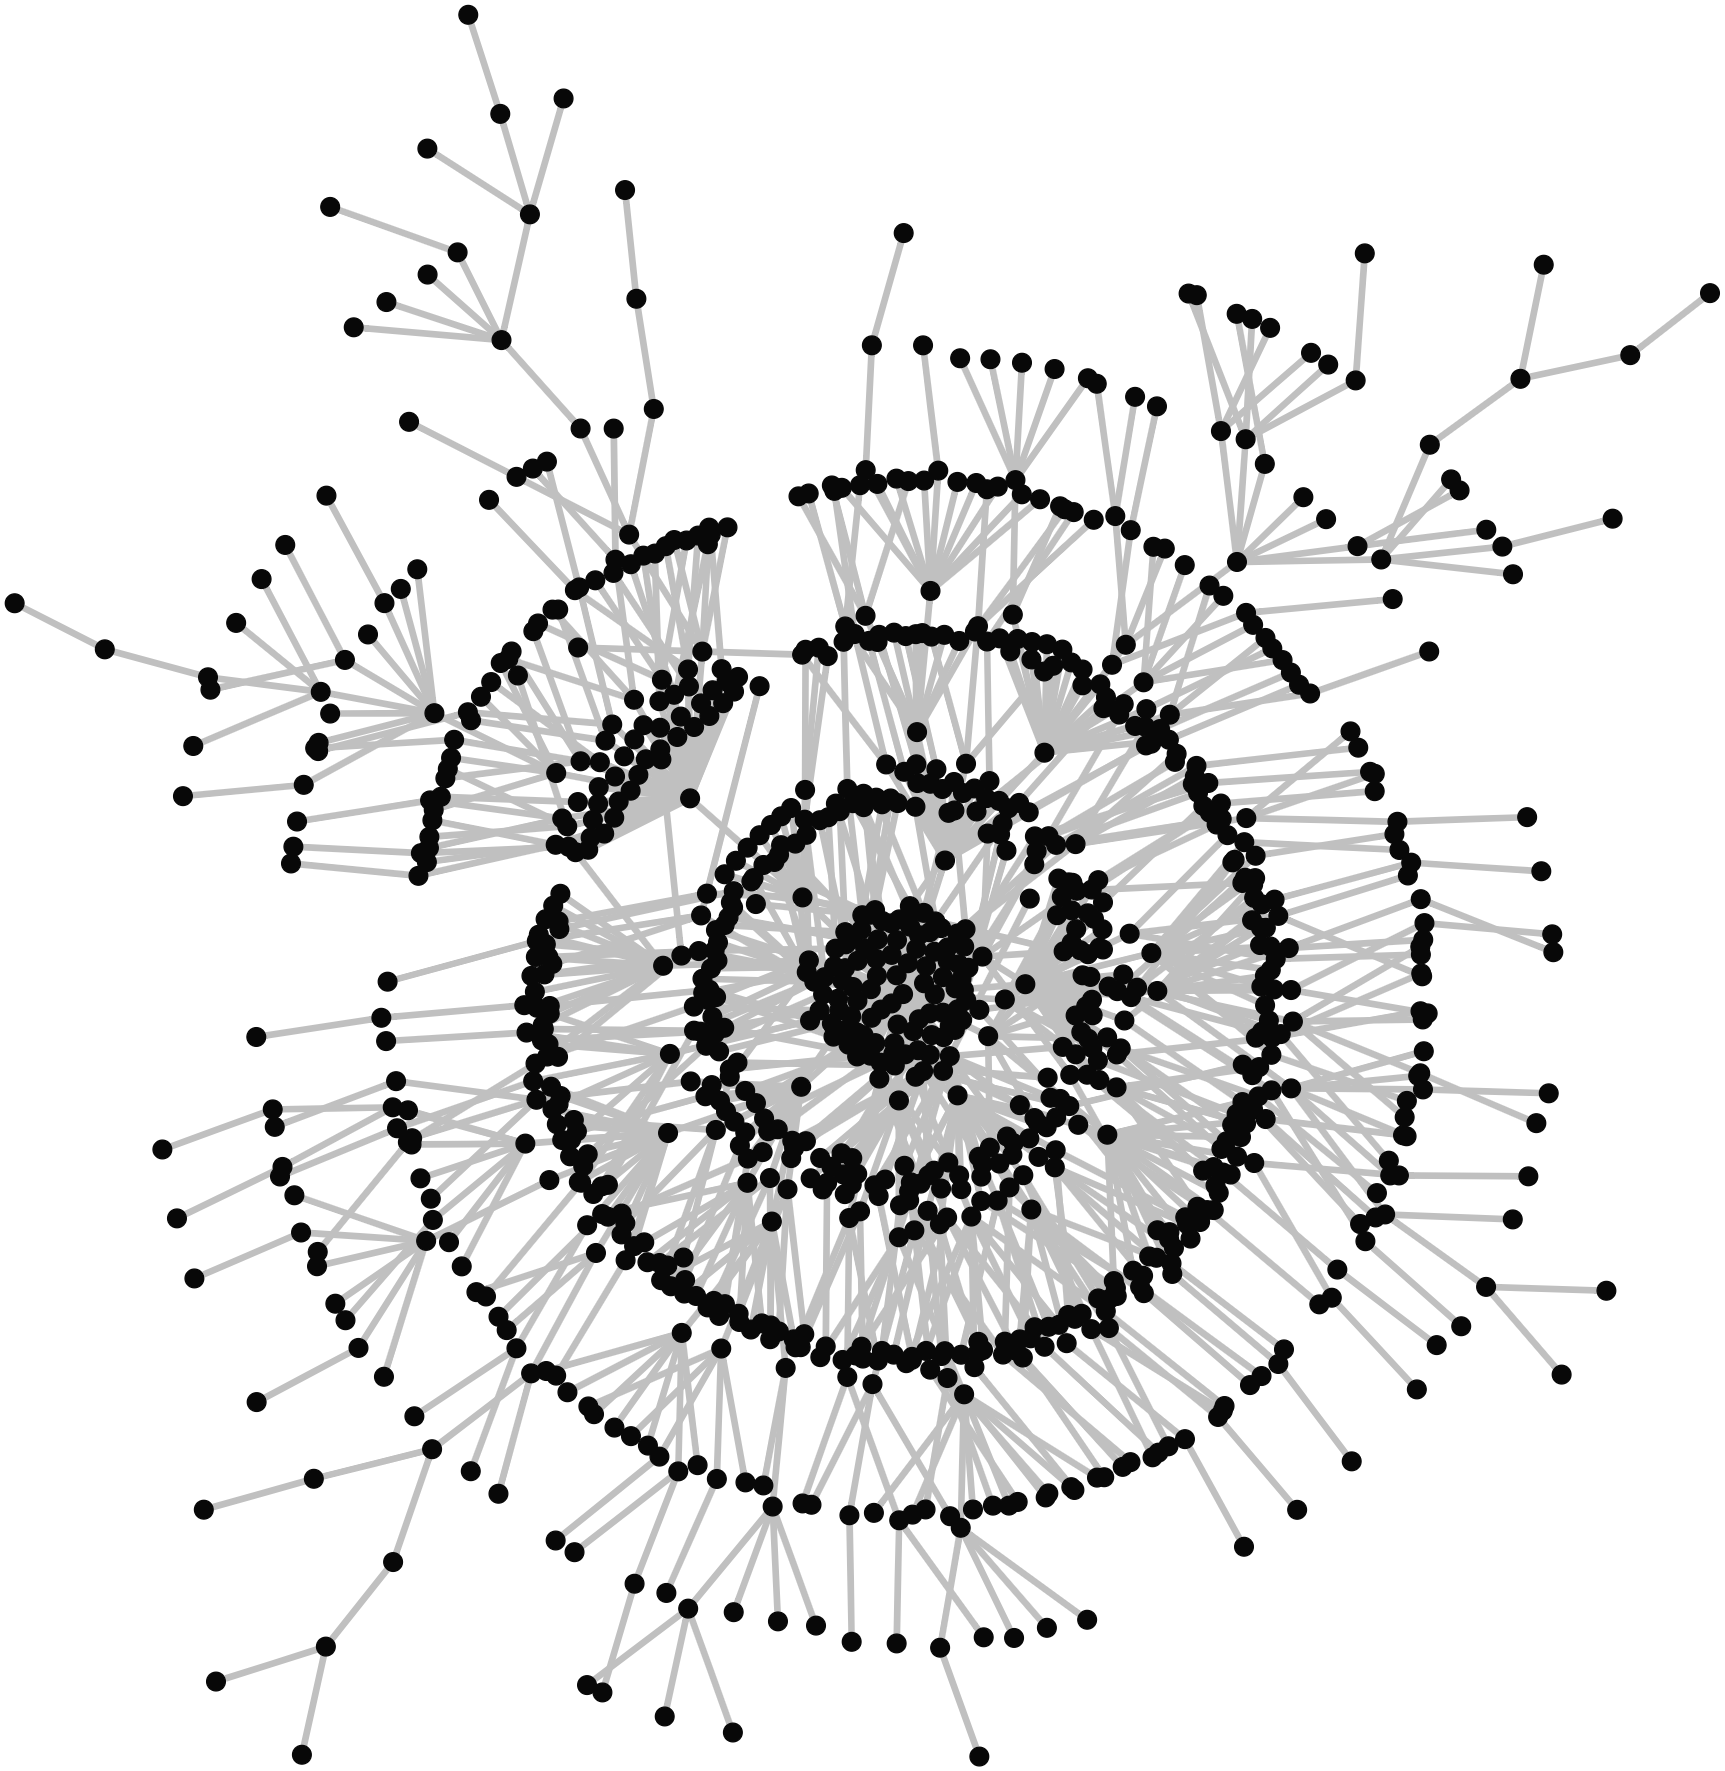
\includegraphics[width=1\linewidth]{images/barabasi_albert_model.png}
    \caption{ Barabási–Albert típusú gráf, $1000$ csomópont. }
    \label{fig:BARABASI_ALBERT_MODEL}
    \vspace{4ex}
  \end{subfigure}%%
  \begin{subfigure}[b]{0.5\linewidth}
    \centering
    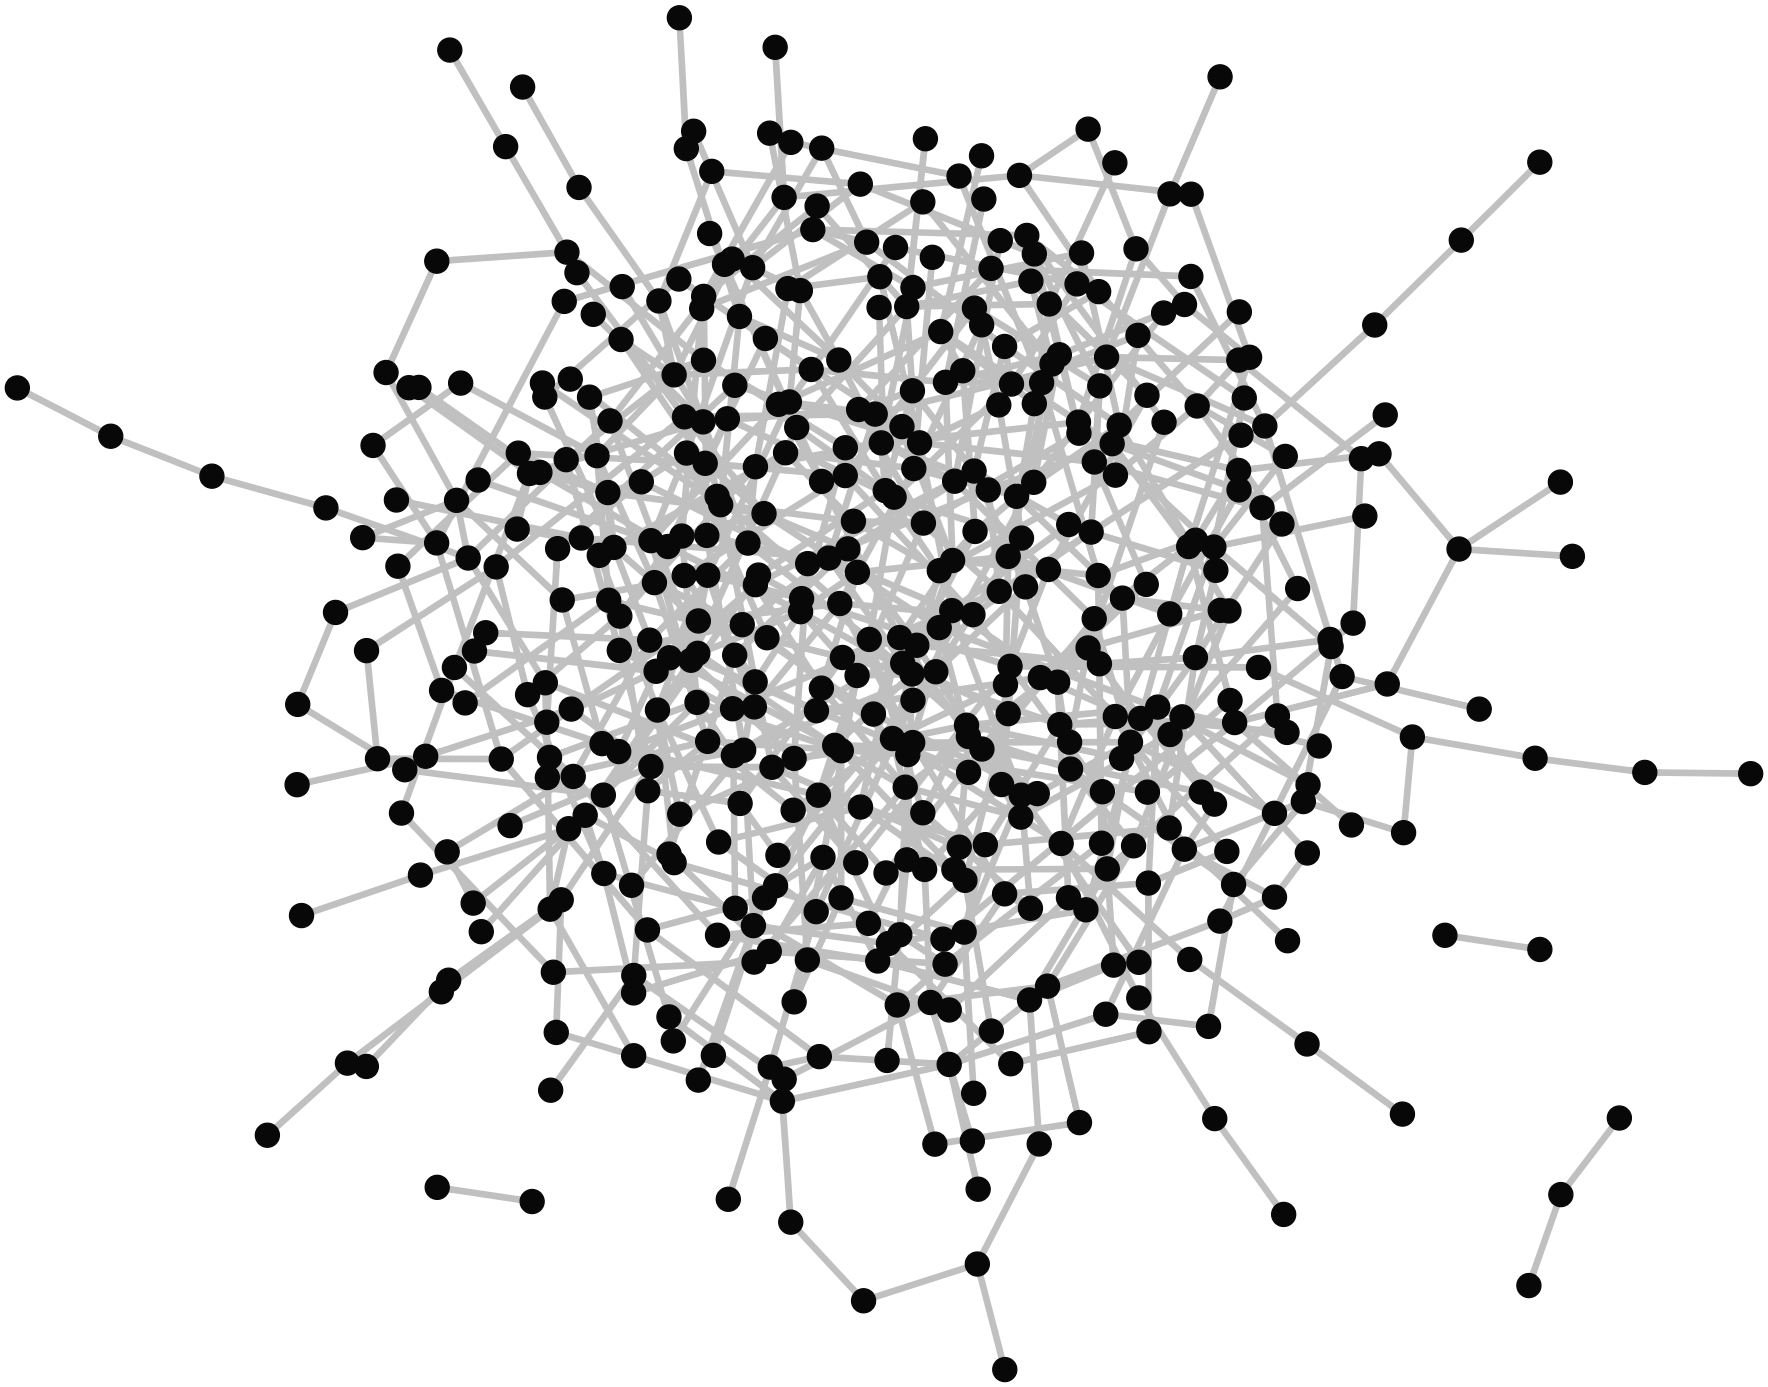
\includegraphics[width=1\linewidth]{images/erdos_renyi_model.png}
    \caption{ Erdős–Rényi típusú gráf, $466$ csomópont. }
    \label{fig:ERDOS_RENYI_MODEL}
    \vspace{4ex}
  \end{subfigure}
  \begin{subfigure}[b]{0.5\linewidth}
    \centering
    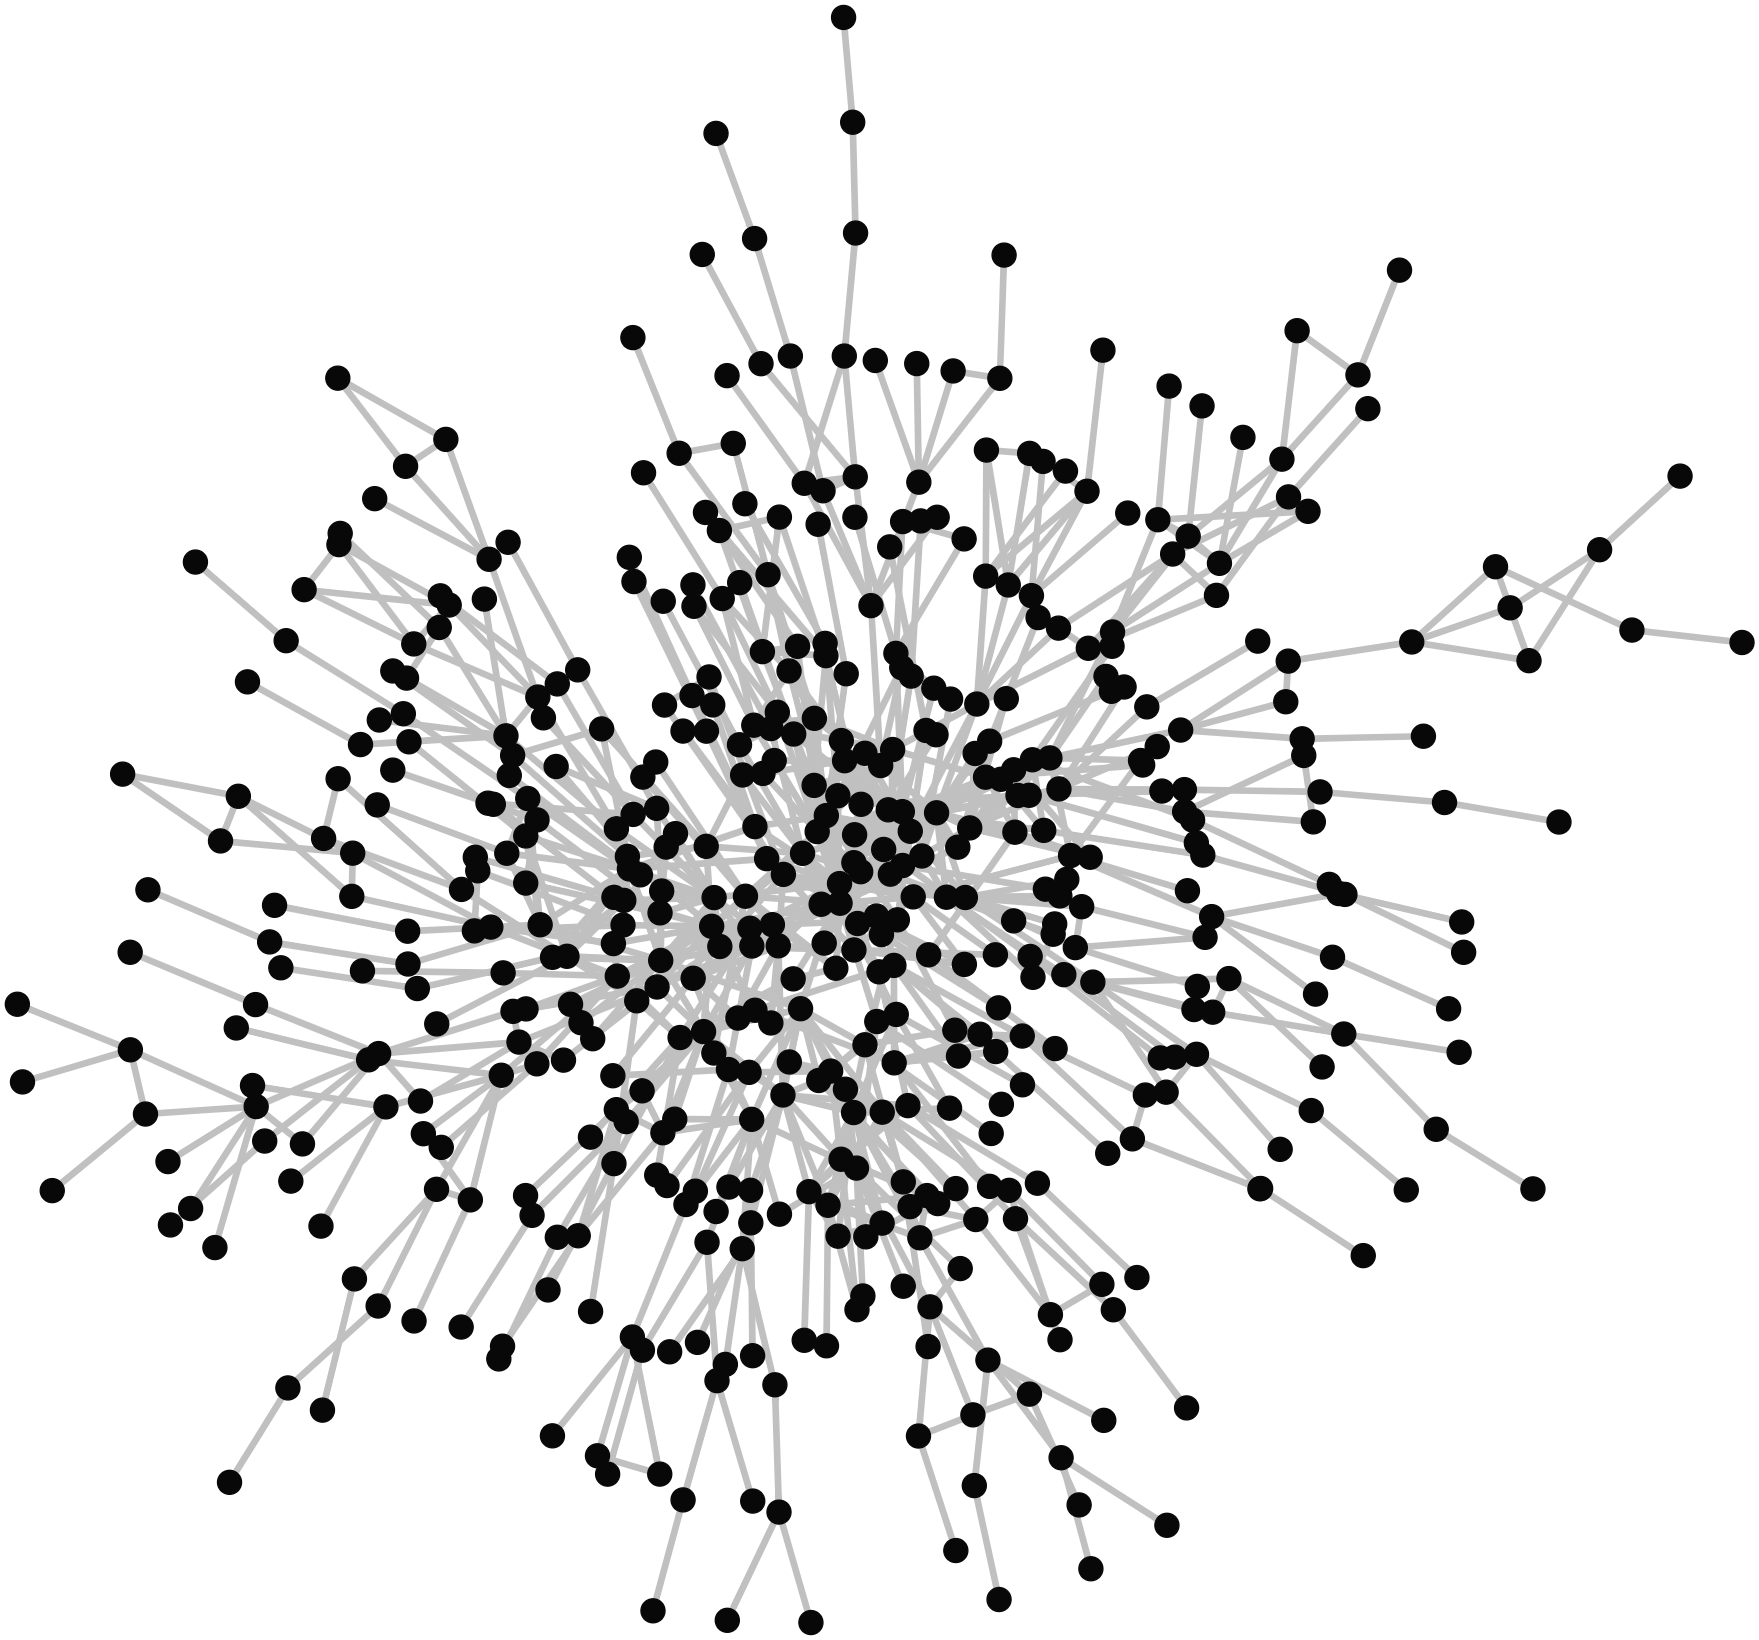
\includegraphics[width=1.15\linewidth]{images/forest_fire_model.png}
    \caption{ Forest-fire típusú gráf, $500$ csomópont. }
    \label{fig:FOREST_FIRE_MODEL}
  \end{subfigure}%%
  \begin{subfigure}[b]{0.5\linewidth}
    \centering
    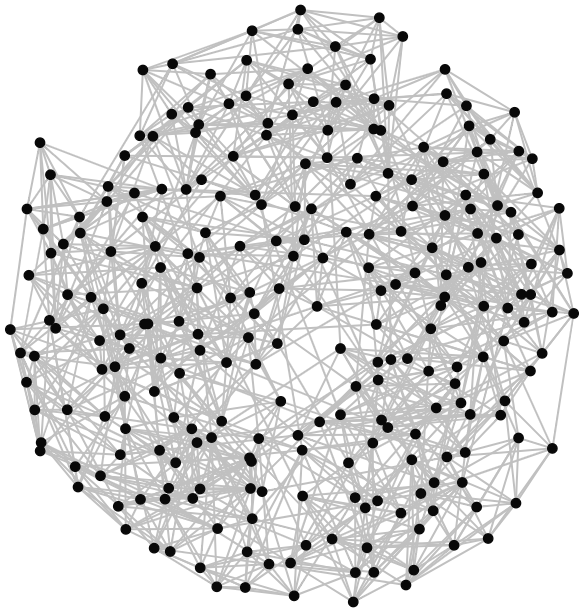
\includegraphics[width=0.85\linewidth]{images/watts_strogatz_model.png}
    \caption{ Watts–Strogatz típusú gráf, $250$ csomópont. }
    \label{fig:WATTS_STROGATZ_MODEL}
  \end{subfigure}\\
  \caption{A bemeneti példányok négy különböző modellje.}
  \label{fig:BENCHMARK_INSTANCES}
\end{figure}
